%
%****************************************************************************************************
%======================= B E G I N   D O C U M E N T   S E T T I N G S ========================
%****************************************************************************************************
%
\documentclass[a4paper, 12pt, xcolor=dvipsnames]{scrartcl}	% Article als Modul
\usepackage[ngerman]{babel}
\usepackage[onehalfspacing]{setspace}
\usepackage{fancyhdr}
\usepackage[usenames, ps2pdf, dvipsnames,svgnames,table]{xcolor}
\usepackage[utf8x]{inputenc}
\usepackage{wrapfig}   
\usepackage{color}
\usepackage[printonlyused, withpage]{acronym}
\usepackage{ifthen}
\usepackage{lastpage}
\usepackage{currfile}
\usepackage{caption}						% Formatierung der Bildunterschriften
\usepackage{sidecap}
\usepackage{subcaption}
\usepackage{tikz}
\usepackage{calc}
\usepackage{graphicx}
\usepackage{multirow}
\usepackage{longtable}
\usepackage{amsthm}
\usepackage{amsbsy}
\usepackage{amssymb}
\usepackage{array}
\usepackage{chngpage}
\usepackage{tabulary} 					% instead of tabularx
\usepackage{array,longtable,calc,amsmath}
\usepackage{xspace}
\usepackage{pdfpages}
\usepackage{textfit}
\usepackage{tabu}
\usepackage{setspace}
\usepackage{listings}
\pagestyle{fancy}
\usepackage[acronym,toc]{glossaries}
\usepackage{docmute}					% includes parts of files just within the Begin and End Document
\usepackage{blindtext}
\usepackage{lipsum}
%---------------------Switch modulare Printversionen
%
\newboolean{UseWm} 		%Korrektur Wasserzeichen in das PDF drucken
\setboolean{UseWm}{false} 		%Zuweisung eines Wertes                    			% Input file für gemeinsame Package Definitionen
%
%--------------------Set data for document:
\newcommand{\SYear}{2021/22}
\newcommand{\SClass}{5AHET}
\newcommand{\ADatum}{04. April 2022}
\newcommand{\DAName}{E$^2$MILY - Elektrische Hardwaredokumentation}
\newcommand{\DPLNameOnePre}{Vorname1}						% Diplomand 1 als Variablenname, usage: \DPLName...
\newcommand{\DPLNameOneSur}{Nachname1}					% Diplomand 1 als Variablenname, usage: \DPLName...
\newcommand{\DPLNameTwoPre}{Vorname2}						% Diplomand 2 als Variablenname, usage: \DPLName...
\newcommand{\DPLNameTwoSur}{Nachname2}					% Diplomand 2 als Variablenname, usage: \DPLName...
\newcommand{\DPLNameThreePre}{Vorname3}					% Diplomand 3 als Variablenname, usage: \DPLName...
\newcommand{\DPLNameThreeSur}{Nachname3}				% Diplomand 3 als Variablenname, usage: \DPLName...
\newcommand{\DPLNameFourPre}{Vorname4}					% Diplomand 4 als Variablenname, usage: \DPLName...
\newcommand{\DPLNameFourSur}{Nachname4}					% Diplomand 4 als Variablenname, usage: \DPLName...
\newcommand{\BNameOnePre}{Vorname1}							% Betreuer 1 als Variablenname, usage: \DPLName...
\newcommand{\BNameOneSur}{Nachname1}						% Betreuer 1 als Variablenname, usage: \DPLName...
\newcommand{\BNameTwoPre}{Vorname2}						% Betreuer 2 als Variablenname, usage: \DPLName...
\newcommand{\BNameTwoSur}{Nachname2}						% Betreuer 2 als Variablenname, usage: \DPLName...
%
\setboolean{UseWm}{true} 												% Wasserzeichen einschalten
%\newcommand{\WatermarkName}{Korrekturexemplar}		%Text für das Wasserzeichen
%\newcommand{\WatermarkName}{01.01.2021}					%AlternativText für das Wasserzeichen
\newcommand{\WatermarkName}{Template}						%AlternativText für das Wasserzeichen
%
%==============================S E T T I N G S ===================================
%
\definecolor{green}{rgb}{0.8,1.0,0.2}
\definecolor{orange}{rgb}{0.9,0.64,0.25}
\definecolor{kaki}{rgb}{0.74,0.74,0.088}
\definecolor{blue}{rgb}{0.2,0.59,0.94}
\definecolor{dred}{rgb}{0.722,0.18,0.18}
\definecolor{htl}{rgb}{0.15625,0.4375,0.507}
%
%------------------------------Watermark wird mit einer Designvariablen geladen ---------------------------------------------------------------------------------
%
\ifthenelse{\boolean{UseWm}}%
{\usepackage{draftwatermark}\SetWatermarkText{\WatermarkName$~-~$\WatermarkName\xspace$~-~$\WatermarkName} \SetWatermarkLightness{0.95}\SetWatermarkScale{0.5}}{}
%
\graphicspath{{./../03_AUX/01_PICT/}}
\newcommand{\changefont}[3]{\fontfamily{#1} \fontseries{#2} \fontshape{#3} \selectfont} % Change a new font
%
% --------------------Set the figure description:
%
\captionsetup{margin=10pt,font=small, labelfont={color=black!80, bf}, textfont={color=black!60}, format=hang, indention=-1cm}
\captionsetup[wrapfigure]{name=Bild}
\captionsetup[figure]{name=Bild}
% --------------------Set the page margins:
%
\setlength{\voffset}{1.0cm}
\setlength{\textwidth}{17.0cm}
%\addtolength{\textheight}{10.0cm}
\setlength{\textheight}{24.0cm}
\setlength{\topmargin }{-2.3cm}
\setlength{\marginparsep }{0pt}
\setlength{\headsep }{1.2cm}
\setlength{\oddsidemargin}{0.0cm}
\setlength{\evensidemargin}{0.0cm}
\setlength{\marginparwidth}{0pt}
\setlength{\hoffset}{-0.54cm}
\setlength{\headwidth}{17.0cm}
\setlength{\footskip}{30pt}
\setlength{\parindent}{0pt}
%
%

%--------------------Set environment for Header and and Footer:
%
\pagestyle{fancy}
\rhead{
\includegraphics[scale=0.06]{/HTL_logo.pdf}}
\chead{}
\lhead{\begin{tabular}{p{12.0cm}} 
\small{\changefont{pag}{b}{sc}\textcolor{black!30}{\DAName}}
\end{tabular} \vspace{0.1cm}}
\lfoot{\small{\changefont{pag}{b}{sc}\textcolor{black!30}{\SYear - \SClass - \DPLNameOneSur, \DPLNameTwoSur, \DPLNameThreeSur, \DPLNameFourSur}}} 
\cfoot{}
\rfoot{\small{\changefont{pag}{b}{sc}\textcolor{black!30}{\thepage\ \textbf{\textcolor{htl!100}I} \pageref{LastPage}}}}
\renewcommand{\headrulewidth}{0.4pt}
\renewcommand{\footrulewidth}{0.4pt}
\let\myHeadrule\headrule
\let\myFootrule\footrule
\renewcommand\headrule{\color{black!30}\myHeadrule }
\renewcommand\footrule{\color{black!30}\myFootrule }
\addto{\captionsngerman}{%
  \renewcommand*{\contentsname}{Inhalt}
  \renewcommand*{\listfigurename}{Abbildungen}
  \renewcommand*{\listtablename}{Abbildungsverzeichnis}
}
%\pagestyle{fancy}
\fancypagestyle{ErsteSeite}{%
   \fancyhf{}%
   \fancyhead[L]{}
}

%\makenoidxglossaries
\renewcommand*\acronymname{Vokabelverzeichnis}
\renewcommand*\glossaryname{Vokabelverzeichnis}

%--------------------Neue Umgebung für M E R K S A T Z:
%
%-------------------- Zählerdefinition:
%
\newcounter{MsNr}
\renewcommand{\theMsNr}{\arabic{MsNr}}
%
\newlength{\boxw}
\newlength{\boxh}
\newlength{\shadowsize}
\newlength{\boxroundness}
\newlength{\tmpa}
\newsavebox{\shadowblockbox}
\setlength{\shadowsize}{6pt}
\setlength{\boxroundness}{3pt}
%
\newenvironment{shadowblock}[1]%
{\begin{lrbox}{\shadowblockbox}\begin{minipage}{#1}}%
{\end{minipage}\end{lrbox}%
\settowidth{\boxw}{\usebox{\shadowblockbox}}%
\settodepth{\tmpa}{\usebox{\shadowblockbox}}%
\settoheight{\boxh}{\usebox{\shadowblockbox}}%
\addtolength{\boxh}{\tmpa}%
\begin{tikzpicture}
\addtolength{\boxw}{\boxroundness * 2}
\addtolength{\boxh}{\boxroundness * 2}
\foreach \x in {0,.05,...,1}
{
\setlength{\tmpa}{\shadowsize * \real{\x}}
\fill[xshift=\shadowsize - 1pt,yshift=-\shadowsize + 
1pt,black,opacity=.04,rounded corners=\boxroundness] 
(\tmpa, \tmpa) rectangle +(\boxw+20 - \tmpa - \tmpa, \boxh+20 - \tmpa - 
\tmpa);
}
\filldraw[fill=yellow!10, draw=kaki!100, rounded corners=\boxroundness] (0, 
0) rectangle (\boxw+20, \boxh+20);
\draw node[xshift=\boxroundness,yshift=\boxroundness,inner sep=10pt,outer 
sep=0pt,anchor=south west] (0,0) {\usebox{\shadowblockbox}};
\end{tikzpicture}}
%
%====================================================================
\newenvironment{Merksatz}
{\begin{shadowblock}{15.8cm}
{\par\vspace*{0.0cm}
\noindent \refstepcounter{MsNr}
\textcolor{kaki!100} {\large{}\textbf{Merke \theMsNr :}} % Hier kann man statt Merke auch etwas anderes hinschreiben
\label{Msl-a}}
}
{\end{shadowblock}}
%
%--------------------End    M E R K S A T Z
% Settings for Codelistings within documentation:
\lstset{ % General setup for the package
	language=C,
	basicstyle=\small\sffamily,
	numbers=left,
 	numberstyle=\tiny,
	frame=tb,
	tabsize=4,
	columns=fixed,
	showstringspaces=false,
	showtabs=false,
	keepspaces,
	commentstyle=\color{red},
	keywordstyle=\color{blue}
}

\setcounter{footnote}{0}

\changefont{pag}{m}{n}                    				% Input file für gemeinsame dokumentenbezogene Definitionen
%
\begin{document}																%ab hier wird der Text im Hauptdokument übernommen
% Verzeichnisse (to be commented out for compilation of main file):
%
%\tableofcontents 																%ACHTUNG: für die Gesamtcompilierung auskommentieren!!
%\newpage 																		%ACHTUNG: für die Gesamtcompilierung auskommentieren!!
%
\changefont{pag}{m}{n}
%
%****************************************************************************************************
%======================== B E G I N  S U B  D O C U M E N T  ==========================
%****************************************************************************************************
%
\section{Diverses}

\subsection{Rahmen}

\fbox{\parbox[0cm][8mm][c]{0cm}{}Hoher Rahmen um einen ganz normalen Text.}\\

\fcolorbox{red}{white}{\parbox[0cm][8mm][c]{0cm}{}Ein hoher roter Rahmen um einen ganz normalen Text.}\\

\fbox{Rahmen um einen ganz normalen Text.}\\

\fcolorbox{red}{white}{Ein roter Rahmen um einen ganz normalen Text.}\\

%----------------------------------------
\Blindtext \lipsum[1-1]	%Blindtext zum Auffüllen mit unsinnigen Sätzen
%----------------------------------------

\pagebreak

\section{Labor oder CPE}
%---------- BEGIN  A u f z ä h l u n g   n u m e r a l  BLAU
\begingroup
\setlength{\LTleft}{-20cm plus -1fill}
\setlength{\LTright}{\LTleft}
	\begin{longtable}[h!]{p{1cm}p{1cm}p{14cm}}
\rowcolor{htl!20}
\multicolumn{3}{l}{\textbf{Sie sollten für diese Übung folgende Vorkenntnisse haben:}}\\
& \dots&Theorie über Ablaufsteuerungen\\
& \dots&Wissen über Zustandsdiagramme und Ablaufketten\\
& \dots&SPS Sprache Ablaufsteuerung\\
&&\\
\rowcolor{htl!20}
\multicolumn{3}{l}{\textbf{Sie lernen in dieser Übung:}}\\
& \dots& Aufgabenstellungen in einem Zustandsdiagramm abzubilden\\
& \dots& wie ein Problem mit einer Ablaufsteuerung gelöst werden kann\\
\end{longtable}
\endgroup
%----------END  A u f z ä h l u n g   n u m e r a l  BLAU
%
%============================== SECTION AUFZÄHLUNGEN
%
\section{Aufzählungen}
%
%================== S U B S E C T I O N
%
\subsection{Punktual}
%---------- BEGIN  A u f z ä h l u n g   p u n k t u a l  m u l t i c o l u m n   l i n e a r 
\begingroup
	\setlength{\LTleft}{-20cm plus -1fill}
	\setlength{\LTright}{\LTleft}
	\begin{longtable}[h!]{p{1.0cm}p{3.0cm}p{9.0cm}}
		\rowcolor{orange!10}
		\multicolumn{3}{l}{\textbf{\parbox[0pt][2em][c]{0cm}{}Aufzählungspunkte mit Spalten linear, Zeilen eingefärbt:}}\\
		\rowcolor{orange!2}
		\includegraphics[width=12pt]{CrossOr} &\textcolor{red!100} {\large\textbf{Schülertext}} &\dots Beschreibung 1.\\
		\rowcolor{orange!6}
		\includegraphics[width=12pt]{CrossGn}&\textcolor{red!100} {\large\textbf{Schülertext}} &\dots Beschreibung 2.\\
		\rowcolor{orange!2}
		\includegraphics[width=12pt]{CrossVi} &\textcolor{red!100} {\large\textbf{Schülertext}} &\dots Beschreibung 1.\\
	\end{longtable}
\endgroup
%---------- END  A u f z ä h l u n g   p u n k t u a l   m u l t i c o l u m n   l i n e a r 
%
%================== S U B S E C T I O N
%
\subsection{Numeral}
%---------- BEGIN  A u f z ä h l u n g   n u m e r a l  m u l t i c o l u m n   l i n e a r 
\begingroup
\setlength{\LTleft}{-20cm plus -1fill}
\setlength{\LTright}{\LTleft}
	\begin{longtable}[h!]{p{1.0cm}p{3.0cm}p{9.0cm}}
		\rowcolor{orange!10}
		\multicolumn{3}{l}{\textbf{\parbox[0pt][2em][c]{0cm}{}Aufzählungsnummerierung mit Spalten linear, Zeilen eingefärbt:}}\\
		\rowcolor{orange!2}
		\includegraphics[width=3mm]{OneOr} &\textcolor{red!100} {\large\textbf{Schülertext}} &\dots Beschreibung 1.\\
		\rowcolor{orange!6}
		\includegraphics[width=3mm]{TwoOr}&\textcolor{red!100} {\large\textbf{Schülertext}} &\dots Beschreibung 2.\\
		\rowcolor{orange!2}
		\includegraphics[width=3mm]{ThreeOr} &\textcolor{red!100} {\large\textbf{Schülertext}} &\dots Beschreibung 3.\\
		\rowcolor{orange!6}
		\includegraphics[width=3mm]{FourOr}&\textcolor{red!100} {\large\textbf{Schülertext}} &\dots Beschreibung 4.\\
		\rowcolor{orange!2}
		\includegraphics[width=3mm]{FiveOr} &\textcolor{red!100} {\large\textbf{Schülertext}} &\dots Beschreibung 5.\\
		\rowcolor{orange!6}
		\includegraphics[width=3mm]{SixOr}&\textcolor{red!100} {\large\textbf{Schülertext}} &\dots Beschreibung 6.\\
		\rowcolor{orange!2}
		\includegraphics[width=3mm]{SevenOr} &\textcolor{red!100} {\large\textbf{Schülertext}} &\dots Beschreibung 7.\\
		\rowcolor{orange!6}
		\includegraphics[width=3mm]{EightOr}&\textcolor{red!100} {\large\textbf{Schülertext}} &\dots Beschreibung 8.\\
		\rowcolor{orange!2}
		\includegraphics[width=3mm]{NineOr} &\textcolor{red!100} {\large\textbf{Schülertext}} &\dots Beschreibung 9.\\
	\end{longtable}
\endgroup
%---------- END  A u f z ä h l u n g   n u m e r a l   m u l t i c o l u m n   l i n e a r 
%---------- BEGIN  A u f z ä h l u n g   n u m e r a l  m u l t i c o l u m n   l i n e a r 
\begingroup
	\setlength{\LTleft}{-20cm plus -1fill}
	\setlength{\LTright}{\LTleft}
	\begin{longtable}[h!]{p{1.0cm}p{3.0cm}p{9.0cm}}
		\rowcolor{orange!10}
		\multicolumn{3}{l}{\textbf{\parbox[0pt][2em][c]{0cm}{}Aufzählungsnummerierung mit Spalten linear, Zeilen eingefärbt:}}\\
		\rowcolor{orange!2}
		\includegraphics[width=3mm]{OneVi} &\textcolor{red!100} {\large\textbf{Schülertext}} &\dots Beschreibung 1.\\
		\rowcolor{orange!6}
		\includegraphics[width=3mm]{TwoGn}&\textcolor{red!100} {\large\textbf{Schülertext}} &\dots Beschreibung 2.\\
	\end{longtable}
\endgroup
%---------- END  A u f z ä h l u n g   n u m e r a l   m u l t i c o l u m n   l i n e a r 
\subsection{OK und NOK}
%---------- BEGIN  T a b e l l e   m i t   O K   u n d   N O K
\begin{center}
	\begin{tabular}{m{3.0cm}m{1.0cm}m{1.0cm}m{1.0cm}m{1.0cm}m{1.0cm}} 
		&\textbf{A} &\textbf{B} & \textbf{C} & \textbf{D} & \textbf{E} \\ 
		\textbf{Text 1:} & \includegraphics[width=0.8cm]{OK} &  & &  &  \\
		\textbf{Text 2:} &  & \includegraphics[width=0.8cm]{NOK} & \includegraphics[width=0.8cm]{OK} & \includegraphics[width=0.8cm]{OK} & \includegraphics[width=0.8cm]{NOK} \\ 
	\end{tabular}
\end{center}
%---------- END  T a b e l l e   m i t   O K   u n d   N O K

%
%================== S U B S E C T I O N
%
\subsection{Multi Table}
%---------- BEGIN  A u f z ä h l u n g    m u l t i t a b l e
%========================================
\vspace{0.5cm}
\begin{longtable}[h!]{p{0.5cm}p{5.2cm}p{9.8cm}}
	\large\textbf{(1)}& \textcolor{red!100} {\large\textbf{Schülertext 1:}}&
\end{longtable}
%========================================
\vspace{-0.5cm}
\begin{longtable}[h!]{p{1.0cm}p{14.5cm}}
	&\textcolor{red!100} {\textbf{Eingerückt 1:}}
\end{longtable}
\vspace{-0.5cm}
\begin{longtable}[h!]{p{2.0cm}p{13.5cm}}
	&Beschreibung Beschreibung Beschreibung Beschreibung Beschreibung Beschreibung Beschreibung Beschreibung Beschreibung. 
\end{longtable}
%========================================
\vspace{-0.5cm}
\begin{longtable}[h!]{p{1.0cm}p{14.5cm}}
	&\textcolor{red!100} {\textbf{Eingerückt 2:}}
\end{longtable}
\vspace{-0.5cm}
\begin{longtable}[h!]{p{2.0cm}p{13.5cm}}
	&Beschreibung Beschreibung Beschreibung Beschreibung Beschreibung Beschreibung Beschreibung Beschreibung Beschreibung.
\end{longtable}
%========================================
\vspace{0.5cm}
\begin{longtable}[h!]{p{0.5cm}p{5.2cm}p{9.8cm}}
	\large\textbf{(2)}& \textcolor{red!100} {\large\textbf{Schülertext 2:}}&
\end{longtable}
%========================================
\vspace{-0.5cm}
\begin{longtable}[h!]{p{1.0cm}p{14.5cm}}
	&\textcolor{red!100} {\textbf{Eingerückt 1:}}
\end{longtable}
\vspace{-0.5cm}
\begin{longtable}[h!]{p{2.0cm}p{13.5cm}}
	&Beschreibung Beschreibung Beschreibung Beschreibung Beschreibung Beschreibung Beschreibung Beschreibung Beschreibung. 
\end{longtable}
%========================================
\vspace{-0.5cm}
\begin{longtable}[h!]{p{1.0cm}p{14.5cm}}
	&\textcolor{red!100} {\textbf{Eingerückt 2:}}
\end{longtable}
\vspace{-0.5cm}
\begin{longtable}[h!]{p{2.0cm}p{13.5cm}}
	&Beschreibung Beschreibung Beschreibung Beschreibung Beschreibung Beschreibung Beschreibung Beschreibung Beschreibung.
\end{longtable}
%---------- END  A u f z ä h l u n g    m u l t i t a b l e

%
%============================== SECTION SUBSECTIONS
%

\section{Subsections}
%
%================== S U B S E C T I O N
%
\subsection{Table in Subsection}
%---------- BEGIN  T a b l e   in  S u b s e c t i o n 
\begin{figure}[h!]
	\begin{minipage}{0.6\textwidth}
		\begin {center}
		\begin{tabular}{|p{2.0cm}|p{3.0cm}|p{1.2cm}|p{1.2cm}|} \hline 
			\textbf{\parbox[0pt][2em][c]{0cm}{}Dezimal$_{10}$} & \textbf{Hexadezimal$_{16}$} & \textbf{Oktal$_{8}$} & \textbf{Dual$_{2}$}\\ \hline 
			0 & 0 & 0 & 0000\\ \hline 
			1 & 1 & 1 & 0001\\ \hline 	
			2 & 2 & 2 & 0010\\ \hline 
			3 & 3 & 3 & 0011\\ \hline 
		\end{tabular}
		\end {center}
    \end{minipage}%\hfill
    \begin{minipage}{0.4\textwidth}
	\linespread {1.25}\changefont{pag}{m}{n}
	Beschreibung Beschreibung Beschreibung Beschreibung.\\
      \caption{Bildbeschreibung Bildbeschreibung Bildbeschreibung.}
	\label{fig:table}
    \end{minipage}
\end{figure}
%---------- END  T a b l e   in  S u b s e c t i o n

%
%================== S U B S E C T I O N
%
\subsection{Text und Graphik in Subsection}
%---------- BEGIN  T e x t   and  G r a p h i k   in  S u b s e c t i o n 
\begin{figure}[h!]
    	\begin{minipage}{0.6\textwidth}
		\begin {center}
		\vspace{0.0cm}
		\centering
		\hspace{-1.0cm}\includegraphics[width=0.8\linewidth]{SecKz_ModKz_Pic_AA}		
		\end {center}
    \end{minipage}%\hfill
    \begin{minipage}{0.4\textwidth}
		\linespread {1.25}\changefont{pag}{m}{n}
		Beschreibung Beschreibung Beschreibung Beschreibung Beschreibung Beschreibung Beschreibung Beschreibung Beschreibung Beschreibung Beschreibung Beschreibung Beschreibung Beschreibung.\\
     		\caption{Bildbeschreibung Bildbeschreibung Bildbeschreibung.}
		\label{fig:SecKz_ModKz_Pic_BB}
    \end{minipage}
\end{figure}
%---------- END  T e x t   and  G r a p h i k    in  S u b s e c t i o n
\pagebreak

%
%============================== SECTION FORMELN
%
\section{Formeln}
%
%================== S U B S E C T I O N
%
\subsection{Lange Formeln}

%----------------------------------------
\lipsum[1-2]\\
%----------------------------------------

%---------- BEGIN   F o r m e l k a s t e n     l a n g
\begin{tabular}[!h]{m{16.4cm}}
	\rowcolor{htl!20}
	Für für eine lange Formel gilt für eine Größe in der Einheit:\\
% Formel:
\color{htl!100}
\begin{center}\large{}\vspace*{-0.2cm}$\begin{aligned}[c]%
%==========
R_{\vartheta 2} &=R_{\vartheta 1} \cdot \left[1+\alpha _{\vartheta 1} \cdot (\vartheta _{2} -\vartheta_1)\right]\\
R_{\vartheta 2} &=R_{20} \cdot \left[1+\alpha _{20} \cdot (\vartheta _{2} -20^{^\circ } C)+\beta_{20} \cdot (\vartheta _{2} -20^{^\circ } C)^2\right]\\
%==========
\end{aligned}$\end{center}
% Erklärung der Formel:
\color{black!70}\changefont{cmr}{m}{it}\begin{spacing}{0.6}\small{\begin{tabbing}
%==========
------\= -------\=-----------------\= \kill %endet mit \kill
$\alpha_{20}$ \>\dots\>linearer Temperaturkoeffizient bei 20$^\circ$C\\
$\beta_{20}$ \>\dots\>quadratischer Temperaturkoeffizient bei 20$^\circ$C\\
$\alpha_{\vartheta 1}$ \>\dots\>linearer Temperaturkoeffizient bei $\vartheta 1$\\
$\beta_{\vartheta 1}$ \>\dots\>quadratischer Temperaturkoeffizient bei $\vartheta 1$\\
$\vartheta_1$ \>\dots\>1. Temperatur des Widerstandes\\
$\vartheta_2$ \>\dots\>2. Temperatur des Widerstandes\\
%==========
\end{tabbing}}\end{spacing}
\vspace{-1.8cm}
\end{tabular}
%---------- END   F o r m e l k a s t e n      l a n g

Text Text Text Text Text Text Text Text Text Text Text Text Text Text Text Text Text Text Text Text Text Text Text Text Text Text Text Text Text Text Text Text Text Text Text Text Text Text Text Text Text Text Text Text Text Text Text Text Text.\\

\subsection{Kurze Formeln}
%----------------------------------------
\Blindtext
%----------------------------------------
$~$\\													%das ist ein unsichtbares Leerzeichen!

%---------- BEGIN   F o r m e l k a s t e n
\begingroup
	\begin{tabular}[!h]{m{6.0cm}m{10.0cm}}
	\rowcolor{htl!20}
	\multicolumn{2}{l}{Für für eine kurze Formel gilt für eine Größe in der Einheit:}\\
% Formel:
\color{htl!100}
\begin{center}
\large{}\vspace*{-0.2cm}
	$\begin{aligned}[c]%
%==========
U_{T} &=\frac{k\cdot T}{q}\approx{26mV}\\
r_{BE} &=\frac{U_{T}}{I_{B}}=\frac{\beta}{S}\\
%==========
	\end{aligned}$
\end{center}
% Erklärung der Formel:
&\color{black!70}\changefont{cmr}{m}{it}\begin{spacing}{0.6}\small{\begin{tabbing}
%==========
------\= -------\=-----------------\= \kill %endet mit \kill
$U_{T}$ \>\dots\>Temperaturspannung $\approx$26mV\\
k \>\dots\>  Boltzmann Konst. k = 1,38$\cdot$10${}^{-23 }$J\textbf{/}K\\
T \>\dots\>  absolute Temperatur in K\\
q \>\dots\>  Einheitsladung mit 1.602$\cdot$10${}^{-}$${}^{19}$${}^{ }$As\\
$r_{BE}$ \>\dots\>  differentieller Basis- Emitterwiderstand\\
$I_{B}$ \>\dots\>  Basisstrom des Transistors\\
${\mathbf \beta }$ \>\dots\>  Stromverstärkung des Transistors
%==========
\end{tabbing}}\end{spacing}
\vspace*{-1.6cm}
	\end{tabular}
\endgroup\\
%---------- END   F o r m e l k a s t e n
Text Text Text Text Text Text Text Text Text Text Text Text Text Text Text Text Text Text Text Text Text Text Text Text Text Text Text Text Text Text Text Text Text Text Text Text Text Text Text Text Text Text Text Text Text Text Text Text Text Text Text Text Text Text Text Text Text Text Text Text Text Text Text Text Text Text.
\pagebreak

%
%============================== SECTION GRAPHIK 
%
\section{Graphik}
%
%================== S U B S E C T I O N
%
\subsection{Wrap Graphik}
%
%---------- BEGIN  W r a p   G r a p h i k
\begin{wrapfigure}[10]{l}{0.45\textwidth} 
	\vspace{-0.5cm}
%\centering
	\includegraphics[width=0.9\linewidth]{SecKz_ModKz_Pic_AA}		
	\hspace{-0.0cm}\caption{Bildunterschrift Wrap Graphik Bildunterschrift Wrap Graphik Bildunterschrift Wrap Graphik Bildunterschrift Wrap Graphik .}
	\label{fig:SecKz_ModKz_Pic_AA}
\end{wrapfigure}
%---------- END  W r a p   G r a p h i k
%
Beschreibung in Bild \ref{fig:SecKz_ModKz_Pic_AA} Beschreibung Beschreibung Beschreibung Beschreibung Beschreibung Beschreibung Beschreibung Beschreibung Beschreibung Beschreibung Beschreibung Beschreibung Beschreibung Beschreibung Beschreibung Beschreibung Beschreibung Beschreibung Beschreibung Beschreibung Beschreibung Beschreibung Beschreibung Beschreibung Beschreibung Beschreibung.
\vspace{2.9cm}

%
%================== S U B S E C T I O N
%
\subsection{Block Graphik}
Text Text Text Text Text Text Text Text Text Text Text Text Text Text Text Text Text Text Text Text Text Text Text Text Text Text Text Text Text Text Text Text Text Text Text Text Text Text Text Text Text Text Text Text Text Text Text Text Text Text Text Text Text Text Text Text Text Text Text Text Text Text Text Text Text Text.\\

%
%---------- BEGIN  B l o c k   G r a p h i k  
\begin{figure}[h!] 
	\vspace{-0.5cm}
%	\centering
	\hspace{-0.0cm}\includegraphics[width=0.25\textwidth]{SecKz_ModKz_Pic_AA}
      \caption{Bildunterschrift Block Graphik Bildunterschrift Block Graphik Bildunterschrift Block Graphik Bildunterschrift Block Graphik.}
	\label{fig:SecKz_ModKz_Pic_AAb}
\end{figure}
%---------- END  B l o c k   G r a p h i k 
%
%----------------------------------------
In Bild \ref{fig:SecKz_ModKz_Pic_AAb} \Blindtext \lipsum[1-2]	%Blindtext zum Auffüllen mit unsinnigen Sätzen
%----------------------------------------
%
\pagebreak

%
%============================== SECTION TABELLEN 
%
\section{Tabellen}

\begin{center}
\begin{tabular}{|p{0.9in}|p{0.5in}|p{0.5in}|p{0.5in}|p{0.5in}|p{0.5in}|p{0.5in}|} \hline 
\multicolumn{2}{|p{1in}|}{} & \multicolumn{2}{|p{0.9in}|}{\textbf{gemessen}} & \multicolumn{3}{|p{1.0in}|}{\textbf{berechnet}} \\ \hline 
\textbf{}\textbf{Mess} & \textbf{f} & \textbf{u${}_{es}$} & \textbf{u${}_{as}$}  & \textbf{A${}_{CL}$} & \textbf{A${}_{CL}$} & \textbf{$\varphi$} \\ \hline 
\textbf{}\textbf{Nr.:} &\textbf{[Hz]} & \textbf{[mV]} & \textbf{[mV]} & \textbf{[-]} & \textbf{[db]}  & \textbf{[${}^\circ$]} \\ \hline 
1 & 1k &  &  &  & &  \\ \hline 
$\dots$& $\dots$& $\dots$& $\dots$&$\dots$&$\dots$&$\dots$ \\ \hline 
10 & 1M &  &  &  &  &\\ \hline 
\end{tabular}
\end{center}
%
%============================== SECTION LERNZIELKONTROLLE 
%

\section{Glossar oder Acronymverzeichnis}
Dies ist ein Text mit einer Abkürzung. Sie können die Buchstabenkombinationen (Kurzzeichen oder Abkürzungen) in der Dokumentation Ihrer \acs{DA} mit einem Befehl aufrufen. Zum Beispiel nehmen wir \acs{ESD}. Im File DA\_04\_ACR.tex muss der entsprechende Eintrag gemacht werden.

\section{PDF Einbindung}
PDF Dokumente können in vielen Gestalten eingebunden sein. Um Platz zu sparen kann man auch 2 A4 Seiten auf A5 verkleinern und quer auf dem Blatt darstellen!\\

Es können bestimmte Seiten auch ausgelassen werden.\\

Achtung Sonderzeichen, wie griechische Symbole können im Preview sonderbar aussehen. Im ACROBAT READER sollte die Darstellung aber wieder in Ordnung sein.

%---------- BEGIN  I N C L U D E       P D F
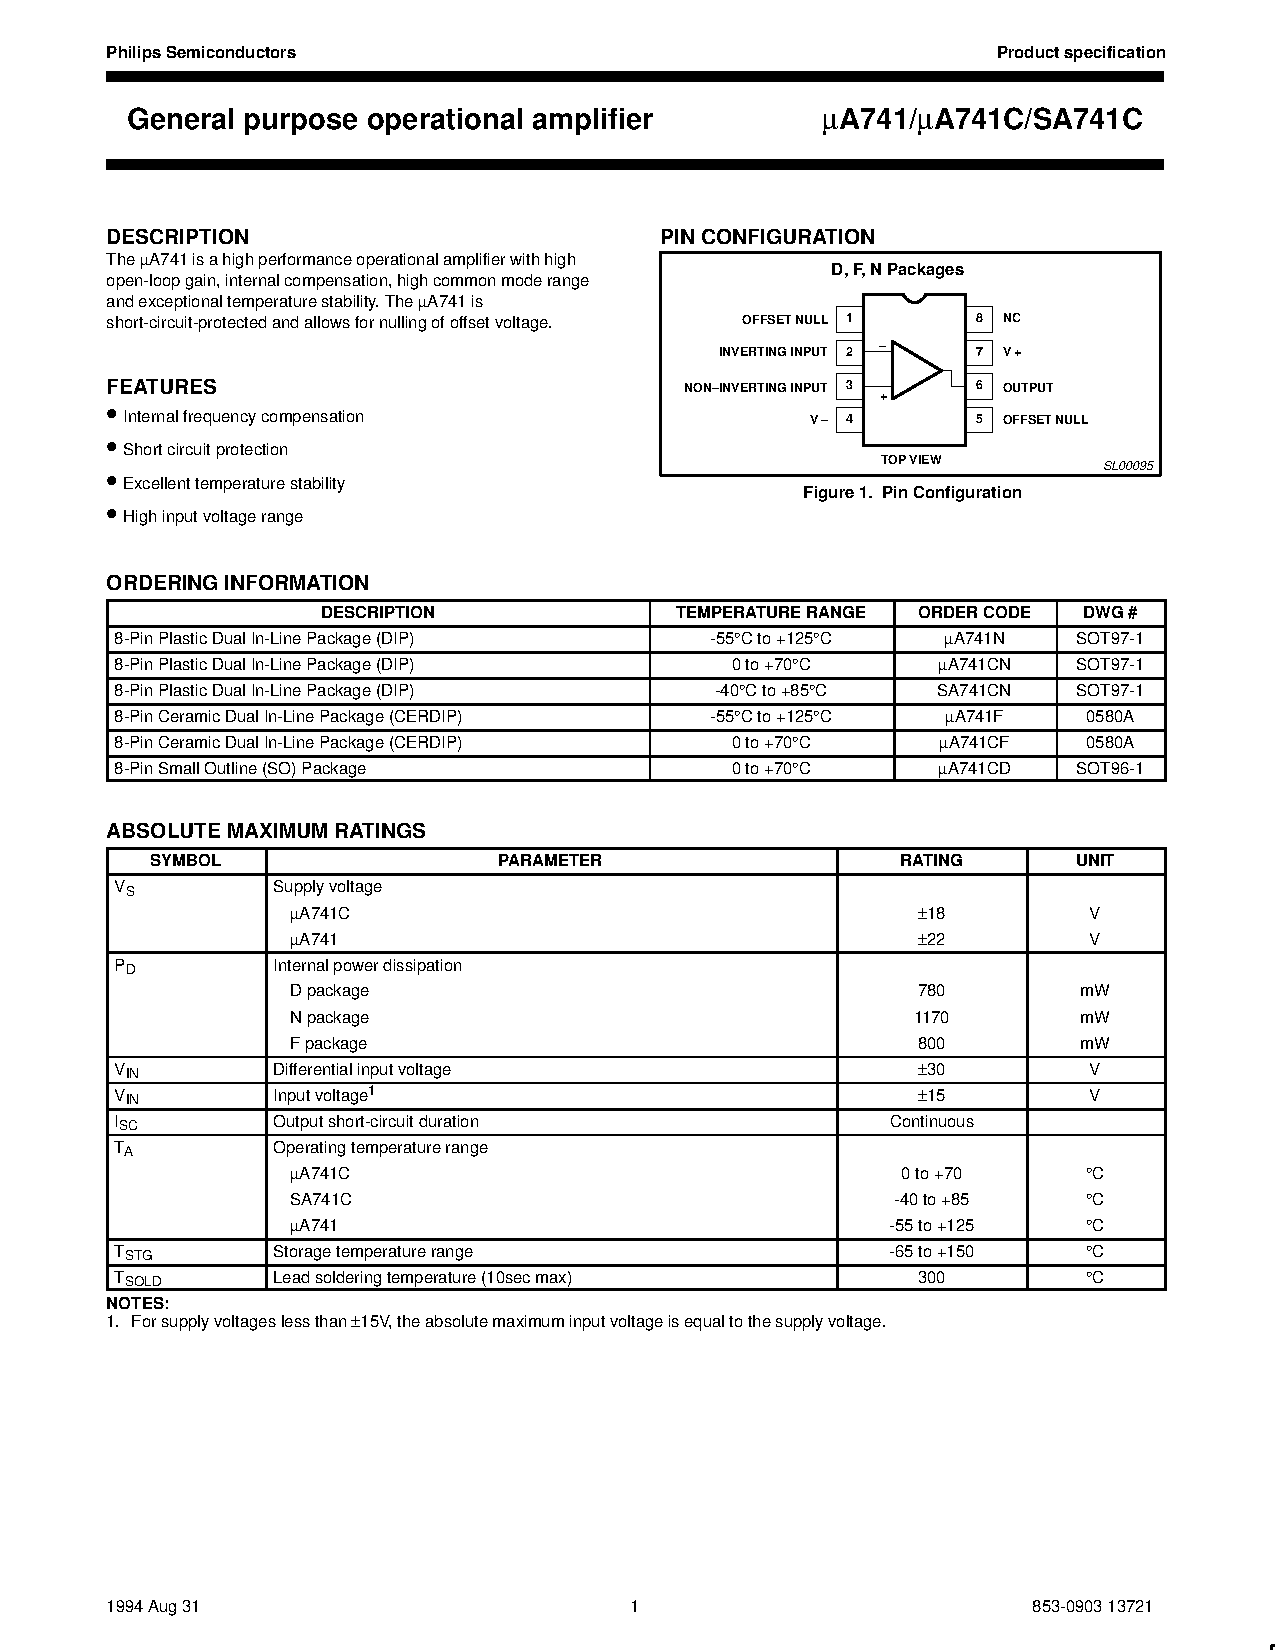
\includepdf[pages={1-6}, nup=1x2, landscape=true]{SecKz_ModKz_Pic_BB.pdf} 
%---------- END  I N C L U D E       P D F
%
%****************************************************************************************************
%============================= E N D   S U B D O C U M E N T  ==========================
%****************************************************************************************************
%
% Verzeichnisse (to be commented out for compilation of main file):
%Im Addendum ist der sogenannte Anhang dargestellt. Beim Verfassen der Dokumentation ist dieser Teil vielleicht noch
%nicht notwendig.
%% Zusammenfassung und Resumee der Diplomarbeit:
\section{Zusammenfassung}

Hier steht die Zusammenfassung und das Resumee der Diplomarbeit!
\newpage

% Anhang zur Diplomarbeit:
\section{Anhang}

Hier stehen zusätzliche Informationen zur Diplomarbeit!
Zum Beispiel können hier Listings oder Teile des Programmes abgebildet sein:

\begin{lstlisting}
// create new document
string path = @"C:\Data\sample.xlsx";
// add title row 
List<string> titleRow = new List<string>();
titleRow.Add("This is the 1st cell");
titleRow.Add("This is the 2nd cell");
openXmlExcel.addTitleRow(titleRow);
// add scatter chart
List<double[]> xValues = new List<double[]>();
List<double[]> yValues = new List<double[]>();
List<string> lineNames = new List<string>();
// first line
xValues.Add(new double[5] { -2, -1, 0, 1, 2 });
yValues.Add(new double[5] { -2, -1, 0, 1, 2 });
lineNames.Add("Line 1");
// second line
xValues.Add(new double[5] { -2, -1, 0, 1, 2 });
yValues.Add(new double[5] { -3, -1, 0, 1, 3 });
lineNames.Add("Line 2");
// save document 
openXmlExcel.saveFile();
\end{lstlisting}

\newpage

\section{Verzeichnisse}
% Bildverzeichnis:
\listoffigures 
%
% Abkürzungsverzeichnis:
%Abkürzungsverzeichnis: Alle Abkürzungen, die bekannt sind finden sich in diesem Verzeichnis.
%Nur diejenigen, die im Dokument auch verwendet werden kommen in die Liste der Compilierung 
%
%der Name der Überschrift kann frei gewählt werden (in diesem Fall: Abkürzungen):
%
%\section*{Acronymverzeichnis}					%Alternative Überschrift für das Verzeichnis
\section*{Abkürzungen}
%
%usage im Dokument: \acs{DA}
%usage im Dokument: \acs{Kurzzeichen}
\begin{acronym}[längstesAcronym]
\setlength{\itemsep}{-0.3 \parsep}
%
% Einträge für Abkürzungen:
%usage im Verzeichnis: \acro{Kurzzeichen}[Inhalt der im Text steht]{Text der als Erklärung im Glossar steht!}
%
\acro{DA}[Diplomarbeit]{Text für die Erklärung der Diplomarbeit}
\acro{ESD}[ESD]{Electrostatic Discharge}
\acro{EMC}[EMC]{Electromagnetic Compatibility}
%
%
% weitere Einträge ...
%
\end{acronym}

%
% Literaturverzeichnis:
%Literaturverzeichnis: Alle Zitate und Veröffentlichungen, die bekannt sind finden sich in diesem Verzeichnis.
%Nur diejenigen, die im Dokument auch verwendet werden kommen in die Liste der Compilierung 
%
%usage im Dokument: \cite{Kurzzeichen}   hier wird im Dokument nur der Text in eckiger Klammer abgebildet
%usage im Dokument: \cite[S~105]{11_Killinger} hier wird auch eine Seitenanzahl dazugestellt
\begin{thebibliography}{22}
%
% Einträge für Literaturverzeichnis:
%usage im Verzeichnis: \bibitem[Werk, Jahrgang oder Auflage]{Kurzzeichen}{Text der als Erklärung im Glossar steht!}
%
   \bibitem[Killinger, 1998]{11_Killinger} Sprache heute : Schriftverkehr; Deutsch für berufsbildende Schulen,\newline 
Seit der Einführung der Bildungsstandards steht der Erwerb fachlicher und sozialer Kompetenzen für Alltag und Beruf im Fokus des Unterrichts.\newline
Autoren: Walter Pirnath, Robert Killinger, Josef Neumüller, 1998
%
\bibitem[vgl. Mustermann, 2020]{12_MM} Skriptum: Test im Zuammenhang mit  ...\newline 
Autoren: Max Mustermann, 2020
%
\bibitem[Werk 1, Jahrgang oder Auflage 1]{BlindzitatKurzzeichen_1}{Text der als Erklärung im Literaturverzeichnis steht!}
%
% weitere Einträge ...
%
\end{thebibliography}
				%ACHTUNG: für die Gesamtcompilierung auskommentieren!!
%Wenn das Addendum auskommentiert ist, dann werden die Zitate im Dokument auch nicht richtig dargestellt.
%Nichts desto Trotz gibt es den Eintrag im Main Dokument auch.
\end{document}


